\chapter{Реализация программного продукта}

В данном разделе приводятся измененный алгоритм поведения Виртуального Актора.

\section{Текущая версия реализованной модели}

Для решения задачи разработки экспериментальной платформы на базе виртуального окружения для изучения социально – эмоционального поведения 
акторов целесообразно использовать специальные программные окружения для разработки виртуальных окружений и сопутствующих компонент – «игровые движки». 
По результатам анализа стало понятно, что такая среда должна прежде всего обладать:
\begin{enumerate}
  \item Большим сообществом разработчиков
  \item Подробной документацией
  \item Относительно низкой сложностью
  \item Простотой установки
  \item Модульной системой
\end{enumerate}

Всеми данными свойствами обладает лишь Unity3D, как самый распространённый, на данный момент инструмент построения виртуальных окружений. 
На базе Unity3D сделано больше игр, чем на любой другой технологии, поэтому он и обладает наиболее развитым сообществом разработчиков на данный момент. 
В сети имеется большое множество документации и курсов по данной технологии. Благодаря модульной системе, можно найти специальные программные модули, 
которые легко встраиваются в разработанный продукт, расширяя возможности всей системы.  Преимуществом данной среды также следует считать относительную 
простоту переноса разработанного виртуального окружения на другие платформы (например, смартфоны, планшеты или же любую из существующих операционных систем). 
Также стоит отметить, что программная среда имеет бесплатную лицензионную версию для небольших команд разработчиков.

Unity предлагает разработчику возможность использовать три различных сценарных языка: C\#, JavaScript (его модификация) и Boo (собственный диалект Python). 
Для разработки данной экспериментальной платформы был выбран C\#, как де факто, стандарт при разработке на Unity3D. 

В качестве среды разработки используется Visual Studio 2019. Для контроля версий использовать облачное хранилище Dropbox и GitLab. 
В качестве средства проектирования использовался стандартный модуль Visual Studio для построения диаграмм классов.

\begin{figure}[h]
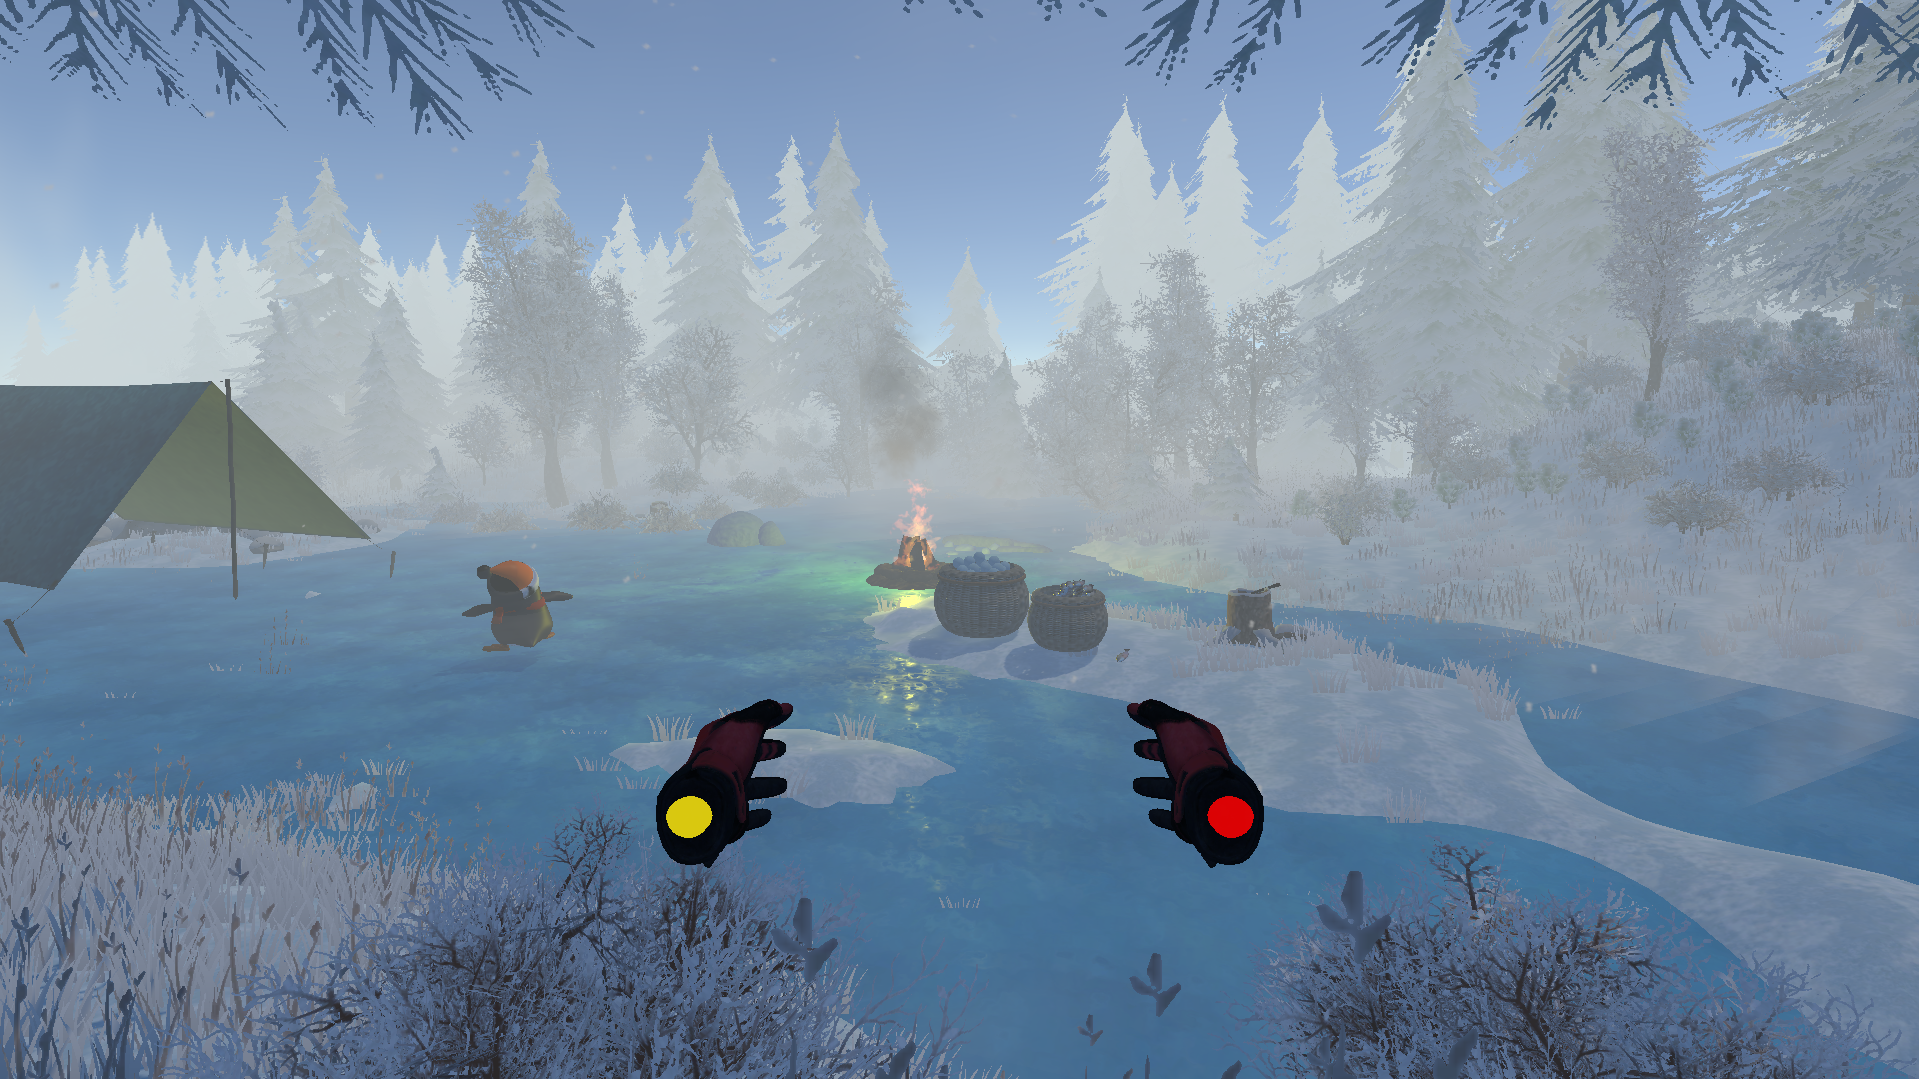
\includegraphics[width=0.75\columnwidth]{./img/penis.png}
\centering
\caption{Cкриншот взаимодействия человека с Виртуальным Актором}
\label{pic:penis}
\end{figure}

В работе было реализовано программное приложени с помощью движка юнити результаты работы которого вы можете видеть на (рис. \ref{pic:penis})

\section{Интеграция моделей из python в C\#}

В расширенной диаграмме классов, было выделено 
какие стадии обработки проходит аудио-запись (Рис. \ref{pic:ncmodel0}).

Получение Audio из UNITY3D осуществлялось при помощи ксласса Microphone и далее помещалось 
в контейнер для аудио данных AudioClip, который хранит аудиофайл либо сжатым в ogg vorbis, либо без сжатия.

Далее, полученная аудио проходит обработку при помощи моделей реализовнных на языке программирования python, 
при непосредственном использовании IronPython, который представляет из себя реализацию языка программирования 
Python с открытым исходным кодом, которая тесно интегрирована с .NET Framework. 
IronPython может использовать библиотеки .NET Framework и Python, а другие языки .NET могут также легко использовать код Python».

Существует несколько методов для работы со скриптами в Ironpython (Рис. \ref{pic:ironpy}):

\begin{figure}[!h]
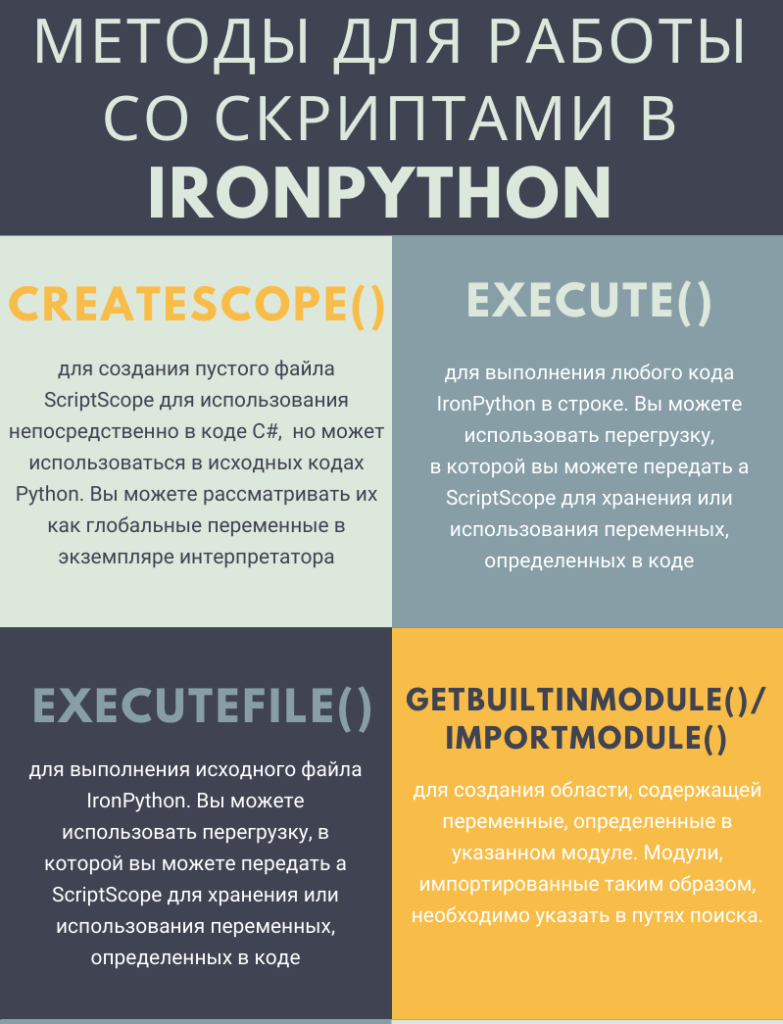
\includegraphics[width=0.40\columnwidth]{./img/ironpy.png}
\centering
\caption{Методы для работы со скриптами в Ironpython}
\label{pic:ironpy}
\end{figure}

Мы использовали метод ExecuteFile(), так как в нашем случае он самый подходящий.

В указанном выше методе проиходит следующее:
\begin{itemize}
  \item В коде C\# в метод ExecuteFile(@"/home/...") помещен путь к файлу .py
  \item Функция из Python определяется в C\#,
  \item Возвращается результат по заврешнию исполнения кода .py,
\end{itemize}

Таким образом проиходит интеграция реализации динамического языка программирования IronPython в проект.


\section{Реализация и дообучение модели}

Как говорилось ранее для создания возможности эмоционального взаимодействия пользователя с виртуальным актором - 
берется предобученная модель "jonatasgrosman/wav2vec2-large-xlsr-53-russian". Данная модель 
работает в состве библеотки huggingsound. На выходе модели для отдельного аудиофайла получаются 512-мерные вектора. 
Далее высчитывается средней вектор, который передается в модели для распознования эмоций.
Используется python3.8 и библиотека машинного обучения pytorch и sklearn.

Для SVC с ядром RBF менялся параметр регурялизации, а именно он принимал значения 1, 10 и 100.


Для k-NN менялось количество соседей от 10 до 40 с шагом в 10.


Для MLP выходной слой не менялся и состоял из 8 нейронов, тогда как количество внутрених слоев менялось от 1 до 3 так,
что количество нейронов в них оставалось неизменным и равным 1024.
В качестве функции активации была выбрана функция гиперболического тангенса.

В результате было получено (рис. \ref{pic:table}):

При обучении датасет разбился на парти в 100 образцов в каждой так, чтобы была возмножность
обучать модели на GPU. Обучение проводилось до 10 эпох так, что результирующей модеью становилась та,
что показывала максимальный результат в какой-либо эпохе.
Так как ставится задача классификации, то в качестве функции потерь используется функция потерь перекрестной энтропии.
В качестве опитимизатора использовался оптимизатор Адам.

\section{Выводы}
Было реализовано приложение позволяющее взаимодействовать с виртуальным окружением, в частности с виртуальным актором. 
Были дообучены модели машинного обучения с целью построения эмоционального взаимодействия. 
Для чего в приложение были интегрированы различные технические средства.